\documentclass[]{article}
\usepackage{lmodern}
\usepackage{amssymb,amsmath}
\usepackage{ifxetex,ifluatex}
\usepackage{fixltx2e} % provides \textsubscript
\ifnum 0\ifxetex 1\fi\ifluatex 1\fi=0 % if pdftex
  \usepackage[T1]{fontenc}
  \usepackage[utf8]{inputenc}
\else % if luatex or xelatex
  \ifxetex
    \usepackage{mathspec}
  \else
    \usepackage{fontspec}
  \fi
  \defaultfontfeatures{Ligatures=TeX,Scale=MatchLowercase}
\fi
% use upquote if available, for straight quotes in verbatim environments
\IfFileExists{upquote.sty}{\usepackage{upquote}}{}
% use microtype if available
\IfFileExists{microtype.sty}{%
\usepackage{microtype}
\UseMicrotypeSet[protrusion]{basicmath} % disable protrusion for tt fonts
}{}
\usepackage[margin=1in]{geometry}
\usepackage{hyperref}
\hypersetup{unicode=true,
            pdftitle={DATA 621 - Discussion 11},
            pdfauthor={Joshua Sturm},
            pdfborder={0 0 0},
            breaklinks=true}
\urlstyle{same}  % don't use monospace font for urls
\usepackage{longtable,booktabs}
\usepackage{graphicx,grffile}
\makeatletter
\def\maxwidth{\ifdim\Gin@nat@width>\linewidth\linewidth\else\Gin@nat@width\fi}
\def\maxheight{\ifdim\Gin@nat@height>\textheight\textheight\else\Gin@nat@height\fi}
\makeatother
% Scale images if necessary, so that they will not overflow the page
% margins by default, and it is still possible to overwrite the defaults
% using explicit options in \includegraphics[width, height, ...]{}
\setkeys{Gin}{width=\maxwidth,height=\maxheight,keepaspectratio}
\IfFileExists{parskip.sty}{%
\usepackage{parskip}
}{% else
\setlength{\parindent}{0pt}
\setlength{\parskip}{6pt plus 2pt minus 1pt}
}
\setlength{\emergencystretch}{3em}  % prevent overfull lines
\providecommand{\tightlist}{%
  \setlength{\itemsep}{0pt}\setlength{\parskip}{0pt}}
\setcounter{secnumdepth}{0}
% Redefines (sub)paragraphs to behave more like sections
\ifx\paragraph\undefined\else
\let\oldparagraph\paragraph
\renewcommand{\paragraph}[1]{\oldparagraph{#1}\mbox{}}
\fi
\ifx\subparagraph\undefined\else
\let\oldsubparagraph\subparagraph
\renewcommand{\subparagraph}[1]{\oldsubparagraph{#1}\mbox{}}
\fi

%%% Use protect on footnotes to avoid problems with footnotes in titles
\let\rmarkdownfootnote\footnote%
\def\footnote{\protect\rmarkdownfootnote}

%%% Change title format to be more compact
\usepackage{titling}

% Create subtitle command for use in maketitle
\newcommand{\subtitle}[1]{
  \posttitle{
    \begin{center}\large#1\end{center}
    }
}

\setlength{\droptitle}{-2em}
  \title{DATA 621 - Discussion 11}
  \pretitle{\vspace{\droptitle}\centering\huge}
  \posttitle{\par}
  \author{Joshua Sturm}
  \preauthor{\centering\large\emph}
  \postauthor{\par}
  \predate{\centering\large\emph}
  \postdate{\par}
  \date{04/19/2018}

\usepackage{booktabs}
\usepackage{longtable}
\usepackage{array}
\usepackage{multirow}
\usepackage[table]{xcolor}
\usepackage{wrapfig}
\usepackage{float}
\usepackage{colortbl}
\usepackage{pdflscape}
\usepackage{tabu}
\usepackage{threeparttable}
\usepackage{threeparttablex}
\usepackage[normalem]{ulem}
\usepackage{makecell}

\begin{document}
\maketitle

\section{Objective}\label{objective}

Your objective is to build multiple linear regression and binary
logistic regression models on the training data to predict the
probability that a person will crash their car and also the amount of
money it will cost if the person does crash their car. You can only use
the variables given to you (or variables that you derive from the
variables provided).

\section{1. Data Exploration}\label{data-exploration}

\subsection{1.1 Import Dataset}\label{import-dataset}

\subsubsection{1.1.1 Data Dictionary}\label{data-dictionary}

\begin{table}[H]
\centering\rowcolors{2}{gray!6}{white}

\resizebox{\linewidth}{!}{\begin{tabular}{lll}
\hiderowcolors
\toprule
Variable Name & Definition & Theoretical Effect\\
\midrule
\showrowcolors
INDEX & Identification Variable (do not use) & None\\
TARGET\_FLAG & Was Car in a crash? 1=YES 0=NO & None\\
TARGET\_AMT & If car was in a crash, what was the cost & None\\
AGE & Age of Driver & Very young people tend to be risky. Maybe very old people also\\
BLUEBOOK & Value of Vehicle & Unknown effect on probability of collision, but probably effect the payout if there is a crash\\
\addlinespace
CAR\_AGE & Vehicle Age & Unknown effect on probability of collision, but probably effect the payout if there is a crash\\
CAR\_TYPE & Type of Car & Unknown effect on probability of collision, but probably effect the payout if there is a crash\\
CAR\_USE & Vehicle Use & Commercial vehicles are driven more, so might increase probability of collision\\
CLM\_FREQ & \# Claims (Past 5 Years) & The more claims you filed in the past, the more you are likely to file in the future\\
EDUCATION & Max Education Level & Unknown effect, but in theory more educated people tend to drive more safely\\
\addlinespace
HOME\_VAL & Home Value & In theory, home owners tend to drive more responsibly\\
HOMEKIDS & \# Children at Home & Unknown effect\\
INCOME & Income & In theory, rich people tend to get into fewer crashes\\
JOB & Job Category & In theory, white collar jobs tend to be safer\\
KIDSDRIV & \# Driving Children & When teenagers drive your car, you are more likely to get into crashes\\
\addlinespace
MSTATUS & Marital Status & In theory, married people drive more safely\\
MVR\_PTS & Motor Vehicle Record Points & If you get lots of traffic tickets, you tend to get into more crashes\\
OLDCLAIM & Total Claims (Past 5 Years) & If your total payout over the past five years was high, this suggests future payouts will be high\\
PARENT1 & Single Parent & Unknown effect\\
RED\_CAR & A Red Car & Urban legend says that red cars (especially red sports cars) are more risky. Is that true?\\
\addlinespace
REVOKED & License Revoked (Past 7 Years) & If your license was revoked in the past 7 years, you probably are a more risky driver.\\
SEX & Gender & Urban legend says that women have less crashes then men. Is that true?\\
TIF & Time in Force & People who have been customers for a long time are usually more safe\\
TRAVTIME & Distance to Work & Long drives to work usually suggest greater risk\\
URBANICITY & Home/Work Area & Unknown\\
YOJ & Years on Job & People who stay at a job for a long time are usually more safe\\
\bottomrule
\end{tabular}}
\rowcolors{2}{white}{white}
\end{table}

\subsection{1.2 Data Structure}\label{data-structure}

\begin{table}[H]
\centering\rowcolors{2}{gray!6}{white}

\resizebox{\linewidth}{!}{\begin{tabular}{lrrrrrrrrrrrrr}
\hiderowcolors
\toprule
  & vars & n & mean & sd & median & trimmed & mad & min & max & range & skew & kurtosis & se\\
\midrule
\showrowcolors
INDEX & 1 & 8161 & 5151.8676633 & 2978.8939616 & 5133.0 & 5151.9306172 & 3841.4166 & 1 & 10302.0 & 10301.0 & 0.0020039 & -1.2034213 & 32.9748900\\
TARGET\_FLAG & 2 & 8161 & 0.2638157 & 0.4407276 & 0.0 & 0.2047787 & 0.0000 & 0 & 1.0 & 1.0 & 1.0716614 & -0.8516462 & 0.0048786\\
TARGET\_AMT & 3 & 8161 & 1504.3246481 & 4704.0269298 & 0.0 & 593.7121106 & 0.0000 & 0 & 107586.1 & 107586.1 & 8.7063034 & 112.2884386 & 52.0712628\\
AGE & 4 & 8155 & 44.7903127 & 8.6275895 & 45.0 & 44.8306513 & 8.8956 & 16 & 81.0 & 65.0 & -0.0289889 & -0.0617020 & 0.0955383\\
BLUEBOOK* & 5 & 8161 & 1283.6185516 & 893.5117428 & 1124.0 & 1259.5665492 & 1132.7064 & 1 & 2789.0 & 2788.0 & 0.2472837 & -1.3624655 & 9.8907352\\
\addlinespace
CAR\_AGE & 6 & 7651 & 8.3283231 & 5.7007424 & 8.0 & 7.9632413 & 7.4130 & -3 & 28.0 & 31.0 & 0.2819531 & -0.7489756 & 0.0651737\\
CAR\_TYPE* & 7 & 8161 & 3.5297145 & 1.9653570 & 3.0 & 3.5371420 & 2.9652 & 1 & 6.0 & 5.0 & -0.0047181 & -1.5165329 & 0.0217555\\
CAR\_USE* & 8 & 8161 & 1.6288445 & 0.4831436 & 2.0 & 1.6610507 & 0.0000 & 1 & 2.0 & 1.0 & -0.5332937 & -1.7158080 & 0.0053482\\
CLM\_FREQ & 9 & 8161 & 0.7985541 & 1.1584527 & 0.0 & 0.5886047 & 0.0000 & 0 & 5.0 & 5.0 & 1.2087985 & 0.2842890 & 0.0128235\\
EDUCATION* & 10 & 8161 & 3.0906752 & 1.4448565 & 3.0 & 3.1133405 & 1.4826 & 1 & 5.0 & 4.0 & 0.1162654 & -1.3799674 & 0.0159939\\
\addlinespace
HOME\_VAL* & 11 & 7697 & 1785.4036638 & 1695.1518106 & 1459.0 & 1639.6773827 & 2161.6308 & 1 & 5106.0 & 5105.0 & 0.4287632 & -1.2442165 & 19.3218121\\
HOMEKIDS & 12 & 8161 & 0.7212351 & 1.1163233 & 0.0 & 0.4971665 & 0.0000 & 0 & 5.0 & 5.0 & 1.3411271 & 0.6489915 & 0.0123571\\
INCOME* & 13 & 7716 & 3040.3326853 & 2029.5206655 & 3024.5 & 3018.5644639 & 2647.1823 & 1 & 6612.0 & 6611.0 & 0.0448688 & -1.2445613 & 23.1045422\\
JOB* & 14 & 7635 & 5.0100851 & 2.4637328 & 5.0 & 5.1375020 & 2.9652 & 1 & 8.0 & 7.0 & -0.3438694 & -1.1576033 & 0.0281961\\
KIDSDRIV & 15 & 8161 & 0.1710575 & 0.5115341 & 0.0 & 0.0252719 & 0.0000 & 0 & 4.0 & 4.0 & 3.3518374 & 11.7801916 & 0.0056624\\
\addlinespace
MSTATUS* & 16 & 8161 & 1.4003186 & 0.4899929 & 1.0 & 1.3754021 & 0.0000 & 1 & 2.0 & 1.0 & 0.4068189 & -1.8347231 & 0.0054240\\
MVR\_PTS & 17 & 8161 & 1.6955030 & 2.1471117 & 1.0 & 1.3138306 & 1.4826 & 0 & 13.0 & 13.0 & 1.3478403 & 1.3754900 & 0.0237675\\
OLDCLAIM* & 18 & 8161 & 552.2714128 & 862.2006829 & 1.0 & 380.3196508 & 0.0000 & 1 & 2857.0 & 2856.0 & 1.3085876 & 0.2461666 & 9.5441372\\
PARENT1* & 19 & 8161 & 1.1319691 & 0.3384779 & 1.0 & 1.0399755 & 0.0000 & 1 & 2.0 & 1.0 & 2.1743561 & 2.7281589 & 0.0037468\\
RED\_CAR* & 20 & 8161 & 1.2913859 & 0.4544287 & 1.0 & 1.2392403 & 0.0000 & 1 & 2.0 & 1.0 & 0.9180255 & -1.1573709 & 0.0050303\\
\addlinespace
REVOKED* & 21 & 8161 & 1.1225340 & 0.3279216 & 1.0 & 1.0281820 & 0.0000 & 1 & 2.0 & 1.0 & 2.3018899 & 3.2991013 & 0.0036299\\
SEX* & 22 & 8161 & 1.5360863 & 0.4987266 & 2.0 & 1.5451064 & 0.0000 & 1 & 2.0 & 1.0 & -0.1446959 & -1.9793056 & 0.0055207\\
TIF & 23 & 8161 & 5.3513050 & 4.1466353 & 4.0 & 4.8402512 & 4.4478 & 1 & 25.0 & 24.0 & 0.8908120 & 0.4224940 & 0.0459012\\
TRAVTIME & 24 & 8161 & 33.4857248 & 15.9083334 & 33.0 & 32.9954051 & 16.3086 & 5 & 142.0 & 137.0 & 0.4468174 & 0.6643331 & 0.1760974\\
URBANICITY* & 25 & 8161 & 1.2045093 & 0.4033673 & 1.0 & 1.1306479 & 0.0000 & 1 & 2.0 & 1.0 & 1.4649406 & 0.1460688 & 0.0044651\\
YOJ & 26 & 7707 & 10.4992864 & 4.0924742 & 11.0 & 11.0711853 & 2.9652 & 0 & 23.0 & 23.0 & -1.2029676 & 1.1773410 & 0.0466169\\
\bottomrule
\end{tabular}}
\rowcolors{2}{white}{white}
\end{table}

The dataset has 23 predictor variables, and 8161 cases. Each case
represents a automotive insurance policy holder. We have a sufficiently
large sample size to perform regression analysis on the data.

\hypertarget{missing-data}{\subsubsection{1.2.1 Missing
Data}\label{missing-data}}

\begin{verbatim}
##       INDEX TARGET_FLAG  TARGET_AMT         AGE    BLUEBOOK     CAR_AGE 
##           0           0           0           6           0         510 
##    CAR_TYPE     CAR_USE    CLM_FREQ   EDUCATION    HOME_VAL    HOMEKIDS 
##           0           0           0           0         464           0 
##      INCOME         JOB    KIDSDRIV     MSTATUS     MVR_PTS    OLDCLAIM 
##         445         526           0           0           0           0 
##     PARENT1     RED_CAR     REVOKED         SEX         TIF    TRAVTIME 
##           0           0           0           0           0           0 
##  URBANICITY         YOJ 
##           0         454
\end{verbatim}

There are several variables that have missing data: \texttt{age},
\texttt{yoj}, \texttt{income}, \texttt{home\_val}, \texttt{job}, and
\texttt{car\_age}. When looking at the data dictionary for the
defintions of these variables, it seems that each of these variables are
independent of each other. For example, some cases have \texttt{yoj}
missing, but may have values for \texttt{job} or \texttt{income}. This
leads me to believe that the missing data is missing at random.
Therefore, I will not remove these cases, but instead try to use some
form of imputation.

\begin{verbatim}
## Observations: 8,161
## Variables: 26
## $ INDEX       <int> 1, 2, 4, 5, 6, 7, 8, 11, 12, 13, 14, 15, 16, 17, 1...
## $ TARGET_FLAG <int> 0, 0, 0, 0, 0, 1, 0, 1, 1, 0, 1, 0, 0, 1, 1, 0, 0,...
## $ TARGET_AMT  <dbl> 0.000, 0.000, 0.000, 0.000, 0.000, 2946.000, 0.000...
## $ AGE         <int> 60, 43, 35, 51, 50, 34, 54, 37, 34, 50, 53, 43, 55...
## $ BLUEBOOK    <fct> $14,230, $14,940, $4,010, $15,440, $18,000, $17,43...
## $ CAR_AGE     <int> 18, 1, 10, 6, 17, 7, 1, 7, 1, 17, 11, 1, 9, 10, 5,...
## $ CAR_TYPE    <fct> Minivan, Minivan, z_SUV, Minivan, z_SUV, Sports Ca...
## $ CAR_USE     <fct> Private, Commercial, Private, Private, Private, Co...
## $ CLM_FREQ    <int> 2, 0, 2, 0, 2, 0, 0, 1, 0, 0, 0, 0, 2, 0, 0, 0, 0,...
## $ EDUCATION   <fct> PhD, z_High School, z_High School, <High School, P...
## $ HOME_VAL    <fct> $0, $257,252, $124,191, $306,251, $243,925, $0, NA...
## $ HOMEKIDS    <int> 0, 0, 1, 0, 0, 1, 0, 2, 0, 0, 0, 0, 0, 0, 0, 3, 0,...
## $ INCOME      <fct> $67,349, $91,449, $16,039, NA, $114,986, $125,301,...
## $ JOB         <fct> Professional, z_Blue Collar, Clerical, z_Blue Coll...
## $ KIDSDRIV    <int> 0, 0, 0, 0, 0, 0, 0, 1, 0, 0, 0, 0, 0, 0, 0, 0, 0,...
## $ MSTATUS     <fct> z_No, z_No, Yes, Yes, Yes, z_No, Yes, Yes, z_No, z...
## $ MVR_PTS     <int> 3, 0, 3, 0, 3, 0, 0, 10, 0, 1, 0, 0, 3, 3, 3, 0, 0...
## $ OLDCLAIM    <fct> $4,461, $0, $38,690, $0, $19,217, $0, $0, $2,374, ...
## $ PARENT1     <fct> No, No, No, No, No, Yes, No, No, No, No, No, No, N...
## $ RED_CAR     <fct> yes, yes, no, yes, no, no, no, yes, no, no, no, no...
## $ REVOKED     <fct> No, No, No, No, Yes, No, No, Yes, No, No, No, No, ...
## $ SEX         <fct> M, M, z_F, M, z_F, z_F, z_F, M, z_F, M, z_F, z_F, ...
## $ TIF         <int> 11, 1, 4, 7, 1, 1, 1, 1, 1, 7, 1, 7, 7, 6, 1, 6, 6...
## $ TRAVTIME    <int> 14, 22, 5, 32, 36, 46, 33, 44, 34, 48, 15, 36, 25,...
## $ URBANICITY  <fct> Highly Urban/ Urban, Highly Urban/ Urban, Highly U...
## $ YOJ         <int> 11, 11, 10, 14, NA, 12, NA, NA, 10, 7, 14, 5, 11, ...
\end{verbatim}

At this point, I usually plot some graphs to better understand the data,
but this dataset is somewhat ``dirty'', and requires tidying before
visualizing it. For this reason, I will include the graphs after
cleaning, which will be done in section 2.

\section{2. Data Preparation}\label{data-preparation}

As can be seen above, the \texttt{\$} character is causing R to classify
what should be numeric columns as characters (and thus factors). I'll
remove all instances of the \texttt{\$} character, as well as the
unnecessary ``z\_'' found in man variables, through the use of regular
expressions.

\subsection{2.1 Remove Extraneous
Characters}\label{remove-extraneous-characters}

\subsection{2.2 Rename Values}\label{rename-values}

\subsection{2.3 Recode Variables}\label{recode-variables}

\subsection{2.4 Data Visualizations}\label{data-visualizations}

\subsubsection{2.4.1 Boxplot}\label{boxplot}

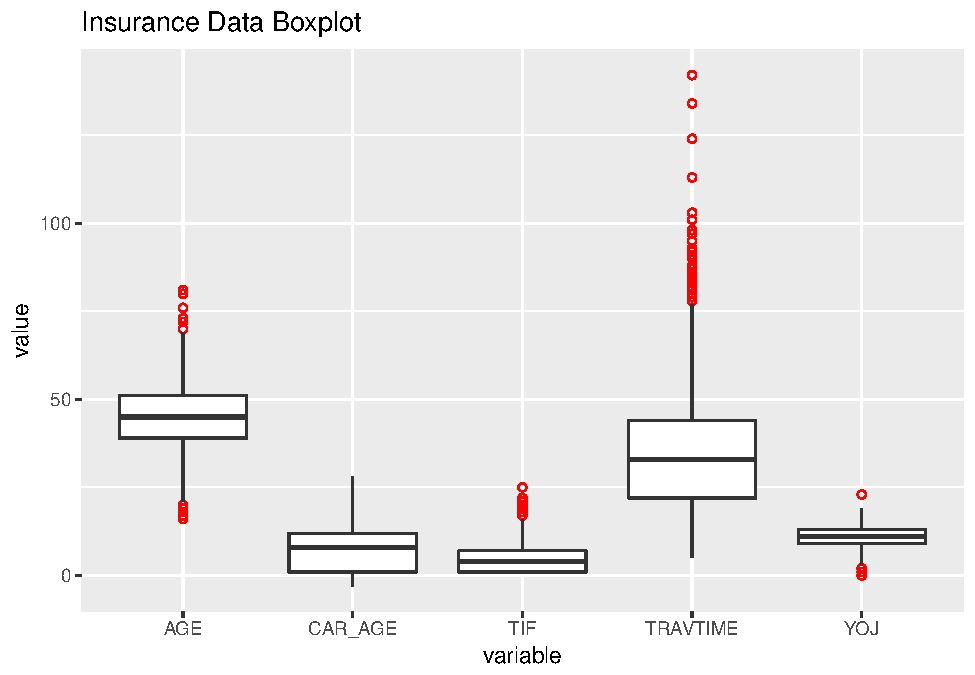
\includegraphics{DATA_621_Homework_4_files/figure-latex/summary-boxplot-1.pdf}
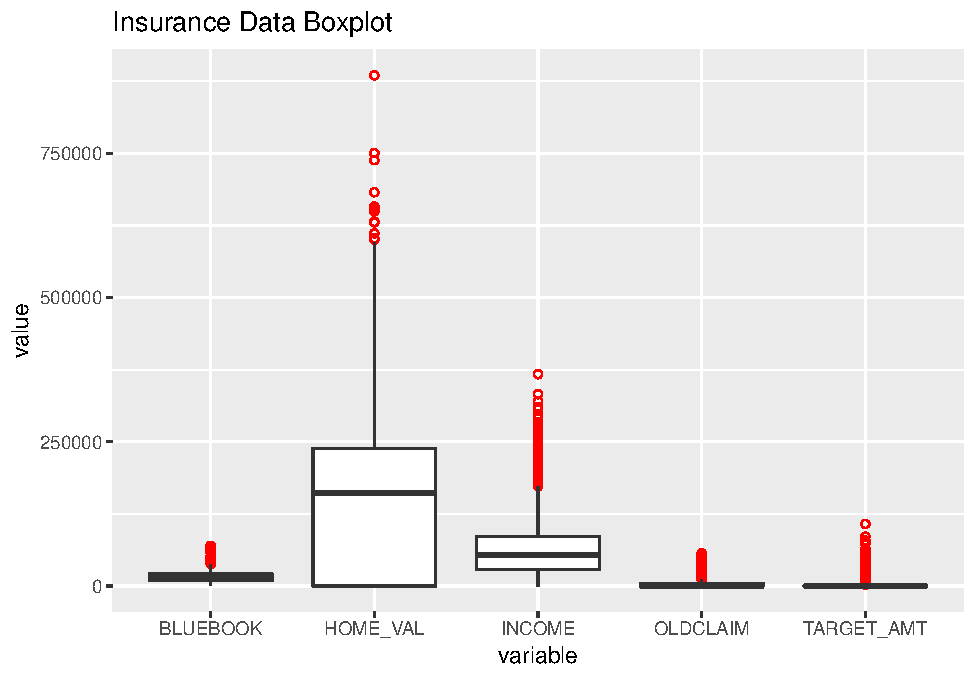
\includegraphics{DATA_621_Homework_4_files/figure-latex/summary-boxplot-2.pdf}

\subsubsection{2.4.2 Histogram}\label{histogram}

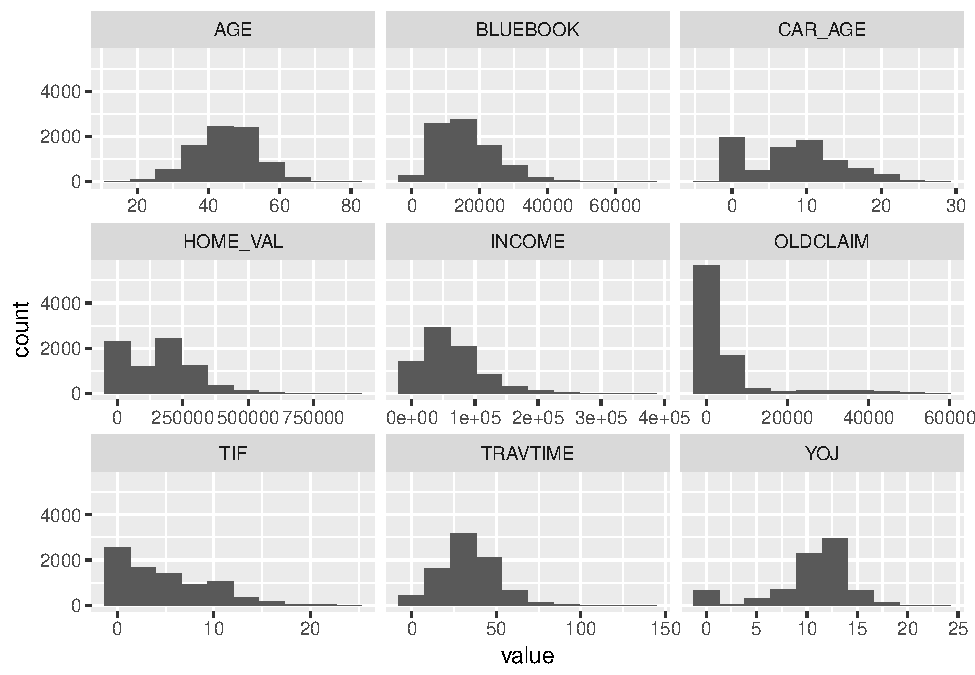
\includegraphics{DATA_621_Homework_4_files/figure-latex/summary-histogram-1.pdf}

From the boxplot and histogram charts, it is much clearer that several
variables are (usally positively) skewed.

\texttt{Age}, \texttt{TIF}, \texttt{TRAVTIME}, \texttt{YOJ},
\texttt{HOME\_VAL}, \texttt{INCOME}, and \texttt{OLDCLAIM} all have
outliers, and are thus strongly skewed.

\subsubsection{2.4.3 Bar Chart}\label{bar-chart}

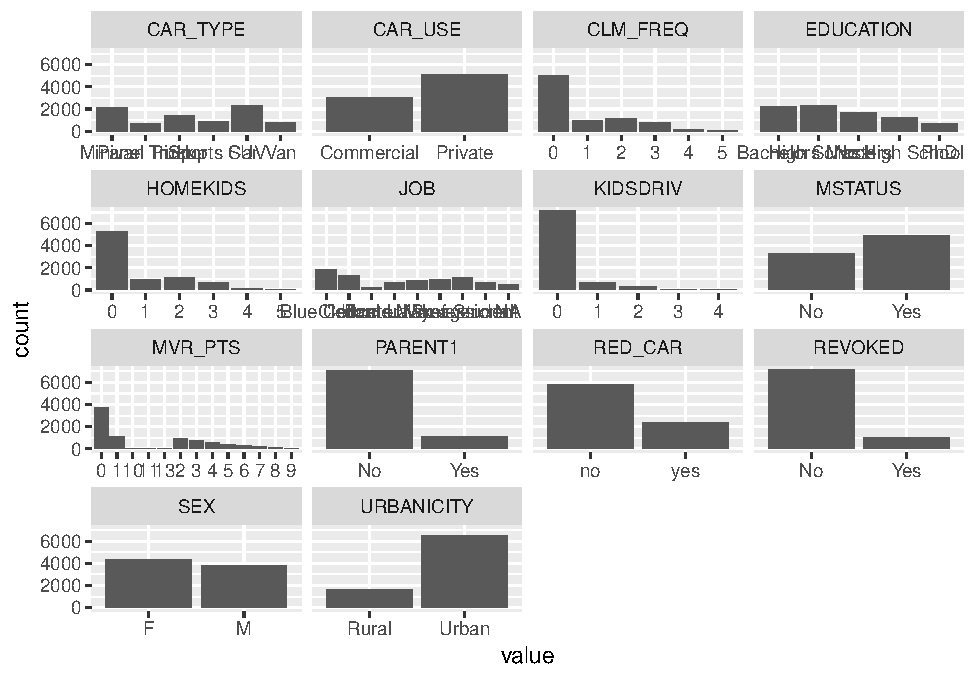
\includegraphics{DATA_621_Homework_4_files/figure-latex/summary-bar-1.pdf}

\subsubsection{2.5 Correlation}\label{correlation}

\paragraph{2.5.1 Correlation Heatmap}\label{correlation-heatmap}

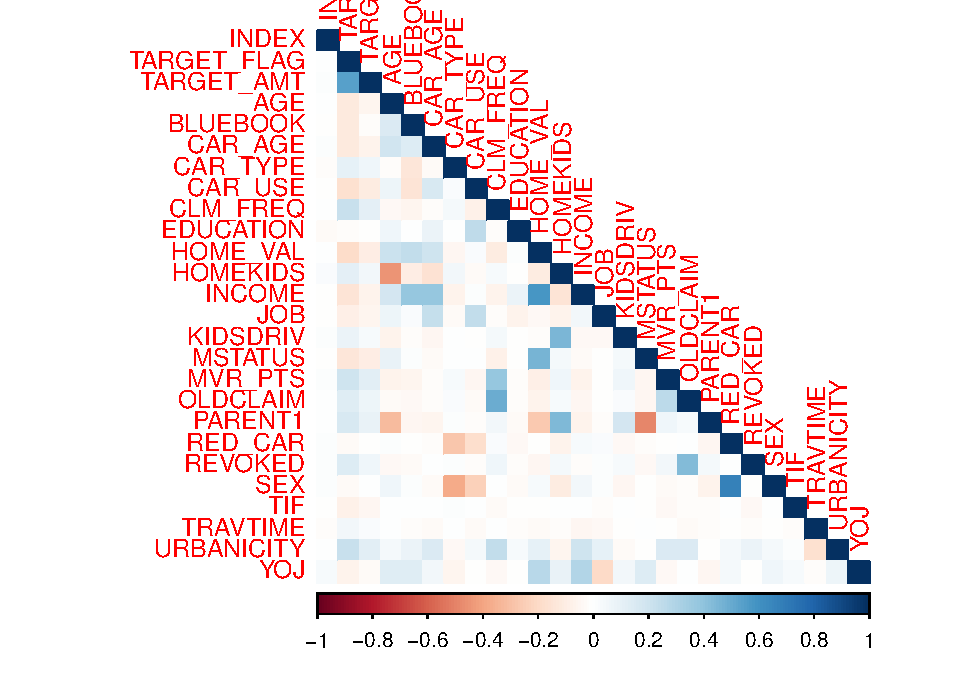
\includegraphics{DATA_621_Homework_4_files/figure-latex/summary-correlation-heatmap-1.pdf}

\paragraph{2.5.2 Correlation (with dependent)
tables}\label{correlation-with-dependent-tables}

\begin{table}[H]
\centering\rowcolors{2}{gray!6}{white}

\resizebox{\linewidth}{!}{\begin{tabular}{lllll}
\hiderowcolors
\toprule
\multicolumn{1}{c}{ } & \multicolumn{2}{c}{TARGET\_FLAG} & \multicolumn{2}{c}{TARGET\_AMT} \\
\cmidrule(l{2pt}r{2pt}){2-3} \cmidrule(l{2pt}r{2pt}){4-5}
  & P-Value & Correlation With Response & P-Value & Correlation With Response\\
\midrule
\showrowcolors
AGE & 2.45719997384773e-19 & -0.115274454488586 & 1.08720017752298e-05 & -0.0565462843235473\\
BLUEBOOK & 3.43696908059188e-18 & -0.111520659047518 & 0.221587047661153 & -0.0157235048062727\\
CAR\_AGE & 8.21488202194266e-18 & -0.110252715120215 & 6.03121914162583e-08 & -0.0696134688694889\\
CAR\_TYPE & 4.53376036668183e-16 & 0.104218255224441 & 2.53297186191568e-06 & 0.0604777749519283\\
CAR\_USE & 3.89464303570401e-36 & -0.160423041105689 & 4.59830665639092e-16 & -0.104196370931591\\
\addlinespace
CLM\_FREQ & 3.96128126250314e-72 & 0.228004364480948 & 8.74826306430675e-19 & 0.113483153860323\\
EDUCATION & 0.376454591569414 & -0.0113775764736867 & 0.706614618574936 & -0.00484224084968468\\
HOME\_VAL & 1.9453233146692e-47 & -0.184515890258562 & 3.02815478688112e-14 & -0.0974998335458788\\
HOMEKIDS & 2.70666614278646e-18 & 0.111865741232024 & 2.86968443947902e-05 & 0.0537804150668685\\
INCOME & 5.78106345956796e-31 & -0.148033809885867 & 1.07195530036848e-06 & -0.0626904470871169\\
\addlinespace
JOB & 1.92037894795254e-11 & -0.0861849678390566 & 4.33463784341559e-05 & -0.0525648622703913\\
KIDSDRIV & 1.28378302025742e-11 & 0.0869333394185601 & 0.00239637636311725 & 0.0390432648967072\\
MSTATUS & 9.76524054228875e-25 & -0.131525287316389 & 3.82263678679032e-13 & -0.0932143897391259\\
MVR\_PTS & 3.54769388013481e-60 & 0.208183430397043 & 5.91899557941683e-23 & 0.126395294702777\\
OLDCLAIM & 2.33133272740956e-27 & 0.138721245102015 & 6.35093636676778e-09 & 0.0746029650375739\\
\addlinespace
PARENT1 & 7.82849941461606e-37 & 0.162017288075898 & 1.23000267660606e-13 & 0.0951543636143193\\
RED\_CAR & 0.0504097542255111 & -0.025164957291153 & 0.78857924023978 & -0.00344967276452347\\
REVOKED & 6.60344427779977e-29 & 0.1427953845581 & 1.87403233389114e-06 & 0.0612615662994889\\
SEX & 0.0619970614539401 & -0.0240057037132183 & 0.832102508818597 & 0.00272733575526047\\
TIF & 8.17234652721987e-10 & -0.0788845226984085 & 0.000633613397170848 & -0.0439341009571584\\
\addlinespace
TRAVTIME & 6.2603210477515e-05 & 0.0514594655005613 & 0.0590375123070895 & 0.024283417647848\\
URBANICITY & 2.55752313377708e-71 & 0.226720968675181 & 4.39351757271654e-22 & 0.123811629456134\\
YOJ & 2.3478393003025e-07 & -0.0664287389752579 & 0.0590092856793026 & -0.0242861213878937\\
\bottomrule
\end{tabular}}
\rowcolors{2}{white}{white}
\end{table}

From the correlation chart and tables, there don't seem to be any
variables correlated one or another with either response variable.
However, there do appear to be several variables related to one another,
although not to the point of extreme collinearity.

\texttt{OLDCLAIM} and \texttt{CLM\_FREQ} have a pearson correlation of
0.4950519. This makes sense, since \texttt{OLDCLAIM} will only have a
value if \texttt{CLM\_FREQ} \(\neq 0\).

\texttt{INCOME} and \texttt{HOME\_VAL} have a pearson correlation of
0.5817192, which is reasonable - a person with a higher salary can
afford a more expensive home, or a home in a more expensive location.

Other correlated variables include: - \texttt{RED\_CAR} and \texttt{SEX}
- \texttt{PARENT1} and \texttt{HOMEKIDS} - \texttt{MSTATUS} and
\texttt{HOME\_VAL}

\subsubsection{2.6 Handling Missing Data}\label{handling-missing-data}

As noted earlier in \protect\hyperlink{missing-data}{Section 1.2.1},
there are several variables with a significant number of missing cases.
I'll break it down by variable, and explain how I will imputate each.

\paragraph{2.6.1 AGE}\label{age}

Each policy holder obviously has an age, and it's most likely required
to be given to the insurer, so this is most likely an error in recording
the data. Since there are so few missing cases, and the variable is
nearly normal, I will impute using the median.

\paragraph{2.6.2 CAR\_AGE}\label{car_age}

Much like the policy holder, ever car also has an age. Since there are
so many missing cases, imputation will be done together with the other
variables via a non-parametric random forest method.

\paragraph{2.6.3 HOME\_VAL}\label{home_val}

There are 464 NA's for this variable. This could be due to recording
errors, or possibly they're equivalent to a 0, meaning the policy holder
doesn't own the home in which they're living. I'll try two different
methods: one where the NA's are converted to a 0, and one imputed via
random forest.

\paragraph{2.6.4 INCOME}\label{income}

This variable has 445 missing cases. Since credit history is an
important factor in insurance premiums, it's likely that income is
required to be declared when creating a new policy. Therefore, like the
other variables, the missing cases could either be due to recording
errors, or simply meant to indicate the applicant had no income. Like
\texttt{HOME\_VAL}, I'll use two different methods to use in separate
models.

\paragraph{2.6.5 JOB}\label{job}

This variable could be missing cases due to the policy holder being
unemployed, or didn't specify their job industry. Imputation will be
handled by the random forest method.

\paragraph{2.6.6 YOJ}\label{yoj}

There are fewer missing values for \texttt{YOJ} than \texttt{JOB}, but
this could be explained by the number of 0 values for \texttt{YOJ},
which could possibly indicate unemployment. Data will be imputated along
with the others via the random forest algorithm.

The algorithm had an error rate of for continuous variables, and for
categorical ones.

\subsubsection{2.7 Variable
Transformation}\label{variable-transformation}

Some of the predictor variables are strongly skewed, and so it may make
sense to either transform them in some way, or simply recode them as
binary variables.

\paragraph{2.7.1 CAR\_AGE}\label{car_age-1}

Firstly, there is a negative value for one of the policy holders, which
is obviously impossible, so I'll assume it was a typographical error,
and use the absolute value, i.e.~3.

Since the majority of cars are \(\leq 1\) year old, I'll recode this to
a binary named \texttt{NEW\_CAR}, with any car \(\geq 1 = 0\).

\paragraph{2.7.2 Remaining Variables}\label{remaining-variables}

The remaining variables with high outliers seem to have reasonable skew.
That is to say, that they're most likely not mistakes in the data, just
extreme cases. In light of this, I will choose to not remove them, as
they may contain information I would not want to lose.

\section{3. Build Models}\label{build-models}

\subsection{3.1 Logistic model}\label{logistic-model}

\subsubsection{3.1.2 Logistic Model One}\label{logistic-model-one}

For the first model, I will use the original dataset, with only the
essential transformations, to use as a baseline with which to compare my
other (modified) datasets.

\begin{verbatim}
## 
## Call:
## glm(formula = TARGET_FLAG ~ . - INDEX - TARGET_AMT, family = binomial(link = "logit"), 
##     data = ins.training)
## 
## Deviance Residuals: 
##     Min       1Q   Median       3Q      Max  
## -2.5837  -0.7001  -0.3848   0.6185   3.1742  
## 
## Coefficients:
##                           Estimate Std. Error z value Pr(>|z|)    
## (Intercept)             -3.027e+00  3.383e-01  -8.950  < 2e-16 ***
## AGE                     -4.228e-05  4.879e-03  -0.009 0.993086    
## BLUEBOOK                -2.238e-05  6.134e-06  -3.649 0.000264 ***
## CAR_AGE                 -3.243e-03  8.969e-03  -0.362 0.717631    
## CAR_TYPEPanel Truck      6.664e-01  1.961e-01   3.398 0.000678 ***
## CAR_TYPEPickup           5.357e-01  1.161e-01   4.613 3.97e-06 ***
## CAR_TYPESports Car       1.109e+00  1.474e-01   7.519 5.50e-14 ***
## CAR_TYPESUV              8.263e-01  1.265e-01   6.530 6.56e-11 ***
## CAR_TYPEVan              5.451e-01  1.508e-01   3.614 0.000302 ***
## CAR_USEPrivate          -8.222e-01  1.067e-01  -7.708 1.27e-14 ***
## CLM_FREQ1                5.847e-01  1.185e-01   4.935 8.00e-07 ***
## CLM_FREQ2                6.538e-01  1.109e-01   5.898 3.68e-09 ***
## CLM_FREQ3                6.539e-01  1.251e-01   5.228 1.71e-07 ***
## CLM_FREQ4                8.441e-01  2.058e-01   4.101 4.12e-05 ***
## CLM_FREQ5                6.065e-01  7.261e-01   0.835 0.403607    
## EDUCATIONHigh School     3.775e-01  1.040e-01   3.629 0.000285 ***
## EDUCATIONMasters        -6.308e-02  1.687e-01  -0.374 0.708534    
## EDUCATIONNo High School  3.925e-01  1.333e-01   2.944 0.003239 ** 
## EDUCATIONPhD             4.865e-01  2.262e-01   2.151 0.031498 *  
## HOME_VAL                -1.360e-06  4.314e-07  -3.152 0.001620 ** 
## HOMEKIDS1                3.842e-01  1.382e-01   2.779 0.005449 ** 
## HOMEKIDS2                2.873e-01  1.361e-01   2.111 0.034811 *  
## HOMEKIDS3                1.222e-01  1.588e-01   0.769 0.441636    
## HOMEKIDS4                3.910e-02  2.479e-01   0.158 0.874665    
## HOMEKIDS5                4.410e-01  7.538e-01   0.585 0.558557    
## INCOME                  -3.426e-06  1.444e-06  -2.373 0.017661 *  
## JOBClerical              1.825e-01  1.211e-01   1.506 0.131953    
## JOBDoctor               -7.250e-01  3.307e-01  -2.192 0.028365 *  
## JOBHome Maker           -1.447e-01  1.792e-01  -0.808 0.419345    
## JOBLawyer                1.769e-02  2.166e-01   0.082 0.934912    
## JOBManager              -8.905e-01  1.615e-01  -5.513 3.53e-08 ***
## JOBProfessional         -9.148e-02  1.377e-01  -0.664 0.506598    
## JOBStudent              -1.746e-01  1.543e-01  -1.131 0.257942    
## KIDSDRIV1                2.849e-01  1.342e-01   2.123 0.033770 *  
## KIDSDRIV2                6.803e-01  1.905e-01   3.572 0.000355 ***
## KIDSDRIV3                8.316e-01  3.524e-01   2.360 0.018294 *  
## KIDSDRIV4               -1.278e+01  3.194e+02  -0.040 0.968089    
## MSTATUSYes              -5.118e-01  1.051e-01  -4.870 1.12e-06 ***
## MVR_PTS1                 8.775e-02  1.073e-01   0.818 0.413286    
## MVR_PTS10                1.015e+00  8.453e-01   1.200 0.229969    
## MVR_PTS11                2.052e+00  1.071e+00   1.917 0.055300 .  
## MVR_PTS13                1.445e+01  3.384e+02   0.043 0.965944    
## MVR_PTS2                 2.633e-01  1.122e-01   2.347 0.018930 *  
## MVR_PTS3                 3.777e-01  1.209e-01   3.124 0.001785 ** 
## MVR_PTS4                 2.834e-01  1.310e-01   2.163 0.030573 *  
## MVR_PTS5                 1.896e-01  1.518e-01   1.249 0.211826    
## MVR_PTS6                 3.745e-01  1.803e-01   2.077 0.037827 *  
## MVR_PTS7                 8.102e-01  2.103e-01   3.852 0.000117 ***
## MVR_PTS8                 1.358e+00  3.404e-01   3.989 6.64e-05 ***
## MVR_PTS9                 1.327e+00  4.009e-01   3.310 0.000935 ***
## OLDCLAIM                -1.919e-05  4.927e-06  -3.895 9.82e-05 ***
## PARENT1Yes               2.257e-01  1.412e-01   1.599 0.109816    
## RED_CARyes              -2.074e-01  1.040e-01  -1.994 0.046133 *  
## REVOKEDYes               9.154e-01  1.094e-01   8.369  < 2e-16 ***
## SEXM                     2.206e-01  1.296e-01   1.702 0.088753 .  
## TIF                     -5.243e-02  8.608e-03  -6.091 1.12e-09 ***
## TRAVTIME                 1.609e-02  2.208e-03   7.288 3.15e-13 ***
## URBANICITYUrban          2.272e+00  1.257e-01  18.078  < 2e-16 ***
## YOJ                     -9.647e-03  9.842e-03  -0.980 0.326969    
## ---
## Signif. codes:  0 '***' 0.001 '**' 0.01 '*' 0.05 '.' 0.1 ' ' 1
## 
## (Dispersion parameter for binomial family taken to be 1)
## 
##     Null deviance: 6990.9  on 6044  degrees of freedom
## Residual deviance: 5319.8  on 5986  degrees of freedom
##   (2116 observations deleted due to missingness)
## AIC: 5437.8
## 
## Number of Fisher Scoring iterations: 12
\end{verbatim}

\paragraph{3.1.2.1 Logistic Model 1
Interpretation}\label{logistic-model-1-interpretation}

The model suggest there are many variables that are not significantly
contributing toward predicting the target variable.

The model has an AIC (Akaike information criterion) of 5437.85, and a
BIC (Bayesian information criterion) of 5833.56.

With a Null deviance of 6990.86, and a Residual deviance of 5319.85, we
get a difference of 1671.01.

Lastly, let's run an ANOVA Chi-Square test to view the effect each
predictor variable is having on the response variable.

\begin{verbatim}
## Analysis of Deviance Table
## 
## Model: binomial, link: logit
## 
## Response: TARGET_FLAG
## 
## Terms added sequentially (first to last)
## 
## 
##            Df Deviance Resid. Df Resid. Dev  Pr(>Chi)    
## NULL                        6044     6990.9              
## AGE         1    80.88      6043     6910.0 < 2.2e-16 ***
## BLUEBOOK    1    56.93      6042     6853.0 4.510e-14 ***
## CAR_AGE     1    39.66      6041     6813.4 3.018e-10 ***
## CAR_TYPE    5   131.28      6036     6682.1 < 2.2e-16 ***
## CAR_USE     1   120.41      6035     6561.7 < 2.2e-16 ***
## CLM_FREQ    5   311.78      6030     6249.9 < 2.2e-16 ***
## EDUCATION   4    31.85      6026     6218.1 2.055e-06 ***
## HOME_VAL    1    78.13      6025     6139.9 < 2.2e-16 ***
## HOMEKIDS    5    34.12      6020     6105.8 2.258e-06 ***
## INCOME      1     0.02      6019     6105.8  0.900818    
## JOB         7    50.17      6012     6055.6 1.335e-08 ***
## KIDSDRIV    4    17.45      6008     6038.2  0.001578 ** 
## MSTATUS     1    37.70      6007     6000.5 8.253e-10 ***
## MVR_PTS    12    71.22      5995     5929.3 1.889e-10 ***
## OLDCLAIM    1     0.04      5994     5929.2  0.851480    
## PARENT1     1     4.36      5993     5924.9  0.036816 *  
## RED_CAR     1     1.27      5992     5923.6  0.260021    
## REVOKED     1   100.09      5991     5823.5 < 2.2e-16 ***
## SEX         1     3.25      5990     5820.3  0.071491 .  
## TIF         1    33.46      5989     5786.8 7.268e-09 ***
## TRAVTIME    1    16.64      5988     5770.2 4.521e-05 ***
## URBANICITY  1   449.35      5987     5320.8 < 2.2e-16 ***
## YOJ         1     0.96      5986     5319.8  0.327035    
## ---
## Signif. codes:  0 '***' 0.001 '**' 0.01 '*' 0.05 '.' 0.1 ' ' 1
\end{verbatim}

\subsubsection{3.1.3 Logistic Model Two}\label{logistic-model-two}

The second model will be using the dataset that was imputated with
zeros.

\begin{verbatim}
## 
## Call:
## glm(formula = TARGET_FLAG ~ . - TARGET_AMT, family = binomial(link = "logit"), 
##     data = insz)
## 
## Deviance Residuals: 
##     Min       1Q   Median       3Q      Max  
## -2.5876  -0.7088  -0.4003   0.6221   3.1751  
## 
## Coefficients:
##                           Estimate Std. Error z value Pr(>|z|)    
## (Intercept)             -3.046e+00  2.793e-01 -10.908  < 2e-16 ***
## AGE                     -9.456e-04  4.016e-03  -0.235 0.813827    
## BLUEBOOK                -2.132e-05  5.258e-06  -4.054 5.03e-05 ***
## NEW_CAR                  8.728e-02  7.637e-02   1.143 0.253130    
## CAR_TYPEPanel Truck      6.011e-01  1.611e-01   3.730 0.000191 ***
## CAR_TYPEPickup           5.609e-01  1.007e-01   5.572 2.51e-08 ***
## CAR_TYPESports Car       1.022e+00  1.298e-01   7.880 3.29e-15 ***
## CAR_TYPESUV              7.695e-01  1.112e-01   6.921 4.47e-12 ***
## CAR_TYPEVan              6.239e-01  1.262e-01   4.945 7.61e-07 ***
## CAR_USEPrivate          -8.057e-01  9.062e-02  -8.891  < 2e-16 ***
## CLM_FREQ                 1.965e-01  2.856e-02   6.879 6.02e-12 ***
## EDUCATIONHigh School     3.927e-01  8.907e-02   4.409 1.04e-05 ***
## EDUCATIONMasters         1.938e-01  1.203e-01   1.611 0.107243    
## EDUCATIONNo High School  3.986e-01  1.128e-01   3.533 0.000410 ***
## EDUCATIONPhD             4.135e-01  1.625e-01   2.545 0.010919 *  
## HOME_VAL                -1.159e-06  3.140e-07  -3.690 0.000224 ***
## HOMEKIDS                 5.597e-02  3.719e-02   1.505 0.132286    
## INCOME                  -2.567e-06  9.737e-07  -2.637 0.008374 ** 
## JOBClerical              1.444e-01  1.064e-01   1.357 0.174694    
## JOBDoctor               -9.274e-01  2.799e-01  -3.313 0.000924 ***
## JOBHome Maker           -4.585e-02  1.525e-01  -0.301 0.763692    
## JOBLawyer               -2.542e-01  1.808e-01  -1.406 0.159797    
## JOBManager              -8.252e-01  1.324e-01  -6.232 4.59e-10 ***
## JOBProfessional         -1.201e-01  1.183e-01  -1.016 0.309822    
## JOBStudent              -5.914e-02  1.290e-01  -0.458 0.646682    
## KIDSDRIV                 3.834e-01  6.114e-02   6.270 3.61e-10 ***
## MSTATUSYes              -5.067e-01  8.160e-02  -6.210 5.30e-10 ***
## MVR_PTS                  1.126e-01  1.362e-02   8.264  < 2e-16 ***
## OLDCLAIM                -1.401e-05  3.915e-06  -3.579 0.000344 ***
## PARENT1Yes               3.804e-01  1.096e-01   3.470 0.000520 ***
## RED_CARyes              -5.334e-03  8.651e-02  -0.062 0.950838    
## REVOKEDYes               8.848e-01  9.134e-02   9.686  < 2e-16 ***
## SEXM                     8.022e-02  1.120e-01   0.716 0.473989    
## TIF                     -5.525e-02  7.345e-03  -7.523 5.37e-14 ***
## TRAVTIME                 1.455e-02  1.884e-03   7.725 1.12e-14 ***
## URBANICITYUrban          2.400e+00  1.129e-01  21.261  < 2e-16 ***
## YOJ                     -1.570e-02  8.598e-03  -1.826 0.067874 .  
## ---
## Signif. codes:  0 '***' 0.001 '**' 0.01 '*' 0.05 '.' 0.1 ' ' 1
## 
## (Dispersion parameter for binomial family taken to be 1)
## 
##     Null deviance: 9418.0  on 8160  degrees of freedom
## Residual deviance: 7296.7  on 8124  degrees of freedom
## AIC: 7370.7
## 
## Number of Fisher Scoring iterations: 5
\end{verbatim}

\paragraph{3.1.3.1 Logistic Model Two
Interpretation}\label{logistic-model-two-interpretation}

This model performed worse than the original one!

The model has an AIC (Akaike information criterion) of 7370.67, and a
BIC (Bayesian information criterion) of 7629.94.

With a Null deviance of 9417.96, and a Residual deviance of 7296.67, we
get a difference of 2121.29.

Lastly, let's run an ANOVA Chi-Square test to view the effect each
predictor variable is having on the response variable.

\begin{verbatim}
## Analysis of Deviance Table
## 
## Model: binomial, link: logit
## 
## Response: TARGET_FLAG
## 
## Terms added sequentially (first to last)
## 
## 
##            Df Deviance Resid. Df Resid. Dev  Pr(>Chi)    
## NULL                        6759     7792.1              
## AGE         1    76.49      6758     7715.7 < 2.2e-16 ***
## BLUEBOOK    1    57.78      6757     7657.9 2.933e-14 ***
## NEW_CAR     1    28.30      6756     7629.6 1.037e-07 ***
## CAR_TYPE    5   144.20      6751     7485.4 < 2.2e-16 ***
## CAR_USE     1   150.14      6750     7335.2 < 2.2e-16 ***
## CLM_FREQ    5   351.08      6745     6984.2 < 2.2e-16 ***
## EDUCATION   4    39.35      6741     6944.8 5.900e-08 ***
## HOME_VAL    1    72.47      6740     6872.3 < 2.2e-16 ***
## HOMEKIDS    5    34.16      6735     6838.2 2.210e-06 ***
## INCOME      1     0.08      6734     6838.1 0.7773687    
## JOB         7    51.82      6727     6786.3 6.348e-09 ***
## KIDSDRIV    4    19.64      6723     6766.6 0.0005876 ***
## MSTATUS     1    50.05      6722     6716.6 1.497e-12 ***
## MVR_PTS    12    86.32      6710     6630.3 2.536e-13 ***
## OLDCLAIM    1     0.13      6709     6630.1 0.7165184    
## PARENT1     1     3.63      6708     6626.5 0.0567129 .  
## RED_CAR     1     0.26      6707     6626.2 0.6106500    
## REVOKED     1   111.75      6706     6514.5 < 2.2e-16 ***
## SEX         1     1.44      6705     6513.0 0.2295195    
## TIF         1    37.56      6704     6475.5 8.862e-10 ***
## TRAVTIME    1    14.24      6703     6461.3 0.0001613 ***
## URBANICITY  1   527.71      6702     5933.5 < 2.2e-16 ***
## YOJ         1     2.26      6701     5931.3 0.1330458    
## ---
## Signif. codes:  0 '***' 0.001 '**' 0.01 '*' 0.05 '.' 0.1 ' ' 1
\end{verbatim}

\subsubsection{3.1.4 Logistic Model Three}\label{logistic-model-three}

For the third logistic model, I will use the dataset that was imputated
via the non-parametric random forest algorithm.

\begin{verbatim}
## 
## Call:
## glm(formula = TARGET_FLAG ~ . - TARGET_AMT, family = binomial(link = "logit"), 
##     data = insrf)
## 
## Deviance Residuals: 
##     Min       1Q   Median       3Q      Max  
## -2.5843  -0.7109  -0.3977   0.6233   3.1680  
## 
## Coefficients:
##                           Estimate Std. Error z value Pr(>|z|)    
## (Intercept)             -2.984e+00  2.855e-01 -10.451  < 2e-16 ***
## X                        4.590e-06  1.238e-05   0.371 0.710872    
## AGE                     -1.057e-03  4.021e-03  -0.263 0.792704    
## BLUEBOOK                -2.091e-05  5.274e-06  -3.965 7.34e-05 ***
## NEW_CAR                  5.424e-02  7.479e-02   0.725 0.468358    
## CAR_TYPEPanel Truck      6.030e-01  1.612e-01   3.740 0.000184 ***
## CAR_TYPEPickup           5.597e-01  1.007e-01   5.559 2.72e-08 ***
## CAR_TYPESports Car       1.018e+00  1.297e-01   7.844 4.37e-15 ***
## CAR_TYPESUV              7.669e-01  1.111e-01   6.901 5.17e-12 ***
## CAR_TYPEVan              6.357e-01  1.263e-01   5.033 4.82e-07 ***
## CAR_USEPrivate          -8.111e-01  9.066e-02  -8.947  < 2e-16 ***
## CLM_FREQ                 1.952e-01  2.856e-02   6.834 8.27e-12 ***
## EDUCATIONHigh School     3.902e-01  8.862e-02   4.403 1.07e-05 ***
## EDUCATIONMasters         2.087e-01  1.206e-01   1.730 0.083668 .  
## EDUCATIONNo High School  3.884e-01  1.130e-01   3.438 0.000585 ***
## EDUCATIONPhD             4.231e-01  1.647e-01   2.568 0.010220 *  
## HOME_VAL                -1.337e-06  3.572e-07  -3.743 0.000182 ***
## HOMEKIDS                 5.448e-02  3.720e-02   1.464 0.143070    
## INCOME                  -3.243e-06  1.140e-06  -2.845 0.004436 ** 
## JOBClerical              1.256e-01  1.068e-01   1.176 0.239506    
## JOBDoctor               -8.740e-01  2.785e-01  -3.138 0.001702 ** 
## JOBHome Maker           -9.718e-02  1.543e-01  -0.630 0.528917    
## JOBLawyer               -2.566e-01  1.811e-01  -1.417 0.156383    
## JOBManager              -7.614e-01  1.317e-01  -5.781 7.43e-09 ***
## JOBProfessional         -1.277e-01  1.189e-01  -1.073 0.283087    
## JOBStudent              -1.187e-01  1.309e-01  -0.907 0.364620    
## KIDSDRIV                 3.796e-01  6.119e-02   6.203 5.53e-10 ***
## MSTATUSYes              -4.807e-01  8.603e-02  -5.588 2.30e-08 ***
## MVR_PTS                  1.136e-01  1.362e-02   8.342  < 2e-16 ***
## OLDCLAIM                -1.388e-05  3.909e-06  -3.550 0.000385 ***
## PARENT1Yes               3.762e-01  1.098e-01   3.427 0.000610 ***
## RED_CARyes              -1.450e-02  8.653e-02  -0.168 0.866931    
## REVOKEDYes               8.911e-01  9.133e-02   9.756  < 2e-16 ***
## SEXM                     8.429e-02  1.120e-01   0.752 0.451887    
## TIF                     -5.547e-02  7.345e-03  -7.551 4.32e-14 ***
## TRAVTIME                 1.457e-02  1.883e-03   7.737 1.02e-14 ***
## URBANICITYUrban          2.394e+00  1.129e-01  21.211  < 2e-16 ***
## YOJ                     -1.494e-02  8.597e-03  -1.738 0.082274 .  
## ---
## Signif. codes:  0 '***' 0.001 '**' 0.01 '*' 0.05 '.' 0.1 ' ' 1
## 
## (Dispersion parameter for binomial family taken to be 1)
## 
##     Null deviance: 9418  on 8160  degrees of freedom
## Residual deviance: 7297  on 8123  degrees of freedom
## AIC: 7373
## 
## Number of Fisher Scoring iterations: 5
\end{verbatim}

\paragraph{3.1.3.1 Logistic Model Three
Interpretation}\label{logistic-model-three-interpretation}

This model performed worse than the original one!

The model has an AIC (Akaike information criterion) of 7372.98, and a
BIC (Bayesian information criterion) of 7639.25.

With a Null deviance of 9417.96, and a Residual deviance of 7296.98, we
get a difference of 2120.99.

Lastly, let's run an ANOVA Chi-Square test to view the effect each
predictor variable is having on the response variable.

\begin{verbatim}
## Analysis of Deviance Table
## 
## Model: binomial, link: logit
## 
## Response: TARGET_FLAG
## 
## Terms added sequentially (first to last)
## 
## 
##            Df Deviance Resid. Df Resid. Dev  Pr(>Chi)    
## NULL                        8160     9418.0              
## X           1     0.02      8159     9417.9 0.8807635    
## AGE         1    87.13      8158     9330.8 < 2.2e-16 ***
## BLUEBOOK    1    65.69      8157     9265.1 5.265e-16 ***
## NEW_CAR     1    26.13      8156     9239.0 3.185e-07 ***
## CAR_TYPE    5   165.39      8151     9073.6 < 2.2e-16 ***
## CAR_USE     1   163.57      8150     8910.0 < 2.2e-16 ***
## CLM_FREQ    1   296.10      8149     8613.9 < 2.2e-16 ***
## EDUCATION   4    50.92      8145     8563.0 2.319e-10 ***
## HOME_VAL    1   124.44      8144     8438.6 < 2.2e-16 ***
## HOMEKIDS    1    31.35      8143     8407.2 2.155e-08 ***
## INCOME      1     0.29      8142     8406.9 0.5927863    
## JOB         7    44.27      8135     8362.7 1.897e-07 ***
## KIDSDRIV    1    34.94      8134     8327.7 3.398e-09 ***
## MSTATUS     1    55.83      8133     8271.9 7.882e-14 ***
## MVR_PTS     1   114.23      8132     8157.6 < 2.2e-16 ***
## OLDCLAIM    1     3.96      8131     8153.7 0.0466456 *  
## PARENT1     1     9.55      8130     8144.1 0.0019952 ** 
## RED_CAR     1     0.16      8129     8144.0 0.6849945    
## REVOKED     1   127.10      8128     8016.9 < 2.2e-16 ***
## SEX         1     0.72      8127     8016.2 0.3974199    
## TIF         1    52.99      8126     7963.2 3.352e-13 ***
## TRAVTIME    1    14.38      8125     7948.8 0.0001494 ***
## URBANICITY  1   648.79      8124     7300.0 < 2.2e-16 ***
## YOJ         1     3.02      8123     7297.0 0.0822852 .  
## ---
## Signif. codes:  0 '***' 0.001 '**' 0.01 '*' 0.05 '.' 0.1 ' ' 1
\end{verbatim}

\subsubsection{3.1.4 Final Logistic Model}\label{final-logistic-model}

Due to the lower AIC, BIC, and deviance values, I will use the second
logistic model for predicting. Note, however, that none of these models
are optimal. From the plots of model two, the residuals are not nearly
normal. This very well could be due to the skewness introduced by the
presence of outliers in the dataset.

\subsection{3.2 Linear Model}\label{linear-model}

I will follow the same format used to build my logistic models for my
linear models.

\subsubsection{3.2.1 Linear Model One}\label{linear-model-one}

\begin{verbatim}
## 
## Call:
## lm(formula = TARGET_AMT ~ . - INDEX - TARGET_FLAG, data = ins.training)
## 
## Residuals:
##    Min     1Q Median     3Q    Max 
##  -7836  -1641   -703    393  82617 
## 
## Coefficients:
##                           Estimate Std. Error t value Pr(>|t|)    
## (Intercept)              2.068e+02  5.381e+02   0.384 0.700764    
## AGE                     -9.958e-01  8.183e+00  -0.122 0.903153    
## BLUEBOOK                 1.329e-02  9.610e-03   1.383 0.166761    
## CAR_AGE                 -2.482e+01  1.448e+01  -1.714 0.086529 .  
## CAR_TYPEPanel Truck      4.262e+02  3.293e+02   1.294 0.195589    
## CAR_TYPEPickup           4.000e+02  1.881e+02   2.126 0.033529 *  
## CAR_TYPESports Car       1.269e+03  2.368e+02   5.357 8.77e-08 ***
## CAR_TYPESUV              9.111e+02  1.949e+02   4.674 3.02e-06 ***
## CAR_TYPEVan              4.936e+02  2.420e+02   2.040 0.041412 *  
## CAR_USEPrivate          -7.394e+02  1.831e+02  -4.038 5.46e-05 ***
## CLM_FREQ1                6.065e+02  2.191e+02   2.769 0.005646 ** 
## CLM_FREQ2                4.091e+02  2.055e+02   1.991 0.046570 *  
## CLM_FREQ3                2.803e+02  2.316e+02   1.211 0.226105    
## CLM_FREQ4                4.433e+02  3.928e+02   1.129 0.259078    
## CLM_FREQ5               -1.562e+02  1.334e+03  -0.117 0.906795    
## EDUCATIONHigh School     1.387e+02  1.746e+02   0.794 0.427019    
## EDUCATIONMasters         6.471e+01  2.512e+02   0.258 0.796694    
## EDUCATIONNo High School  3.628e+02  2.268e+02   1.600 0.109751    
## EDUCATIONPhD             8.142e+02  3.550e+02   2.293 0.021855 *  
## HOME_VAL                -9.728e-04  7.156e-04  -1.359 0.174063    
## HOMEKIDS1                3.321e+02  2.321e+02   1.431 0.152469    
## HOMEKIDS2                4.593e+02  2.276e+02   2.018 0.043646 *  
## HOMEKIDS3                7.101e+00  2.630e+02   0.027 0.978462    
## HOMEKIDS4               -1.409e+02  4.311e+02  -0.327 0.743868    
## HOMEKIDS5                5.841e+02  1.339e+03   0.436 0.662714    
## INCOME                  -2.871e-03  2.289e-03  -1.254 0.209858    
## JOBClerical             -1.750e+02  2.100e+02  -0.833 0.404679    
## JOBDoctor               -1.343e+03  4.978e+02  -2.699 0.006983 ** 
## JOBHome Maker           -2.520e+02  3.006e+02  -0.838 0.401876    
## JOBLawyer               -2.319e+02  3.410e+02  -0.680 0.496561    
## JOBManager              -1.081e+03  2.564e+02  -4.217 2.52e-05 ***
## JOBProfessional         -8.677e+00  2.336e+02  -0.037 0.970374    
## JOBStudent              -4.237e+02  2.650e+02  -1.599 0.109898    
## KIDSDRIV1                4.043e+02  2.355e+02   1.717 0.086098 .  
## KIDSDRIV2                1.461e+02  3.377e+02   0.433 0.665295    
## KIDSDRIV3                5.846e+02  6.496e+02   0.900 0.368201    
## KIDSDRIV4               -2.432e+03  3.160e+03  -0.770 0.441480    
## MSTATUSYes              -6.212e+02  1.710e+02  -3.633 0.000282 ***
## MVR_PTS1                 6.826e+01  1.711e+02   0.399 0.689947    
## MVR_PTS10                5.139e+03  1.474e+03   3.487 0.000492 ***
## MVR_PTS11                1.089e+03  1.399e+03   0.778 0.436623    
## MVR_PTS13                1.266e+03  3.116e+03   0.406 0.684587    
## MVR_PTS2                 4.514e+02  1.875e+02   2.408 0.016073 *  
## MVR_PTS3                 1.728e+02  2.092e+02   0.826 0.409052    
## MVR_PTS4                 2.605e+02  2.342e+02   1.112 0.266103    
## MVR_PTS5                 9.103e+02  2.829e+02   3.218 0.001297 ** 
## MVR_PTS6                 5.112e+02  3.399e+02   1.504 0.132615    
## MVR_PTS7                 6.781e+02  4.062e+02   1.670 0.095063 .  
## MVR_PTS8                 2.221e+03  6.191e+02   3.587 0.000337 ***
## MVR_PTS9                 2.653e+03  7.150e+02   3.711 0.000209 ***
## OLDCLAIM                -1.269e-02  8.976e-03  -1.414 0.157387    
## PARENT1Yes               2.335e+02  2.426e+02   0.962 0.335900    
## RED_CARyes              -1.527e+02  1.711e+02  -0.892 0.372336    
## REVOKEDYes               5.657e+02  1.975e+02   2.865 0.004188 ** 
## SEXM                     4.851e+02  2.039e+02   2.379 0.017389 *  
## TIF                     -4.524e+01  1.369e+01  -3.305 0.000956 ***
## TRAVTIME                 1.093e+01  3.615e+00   3.022 0.002521 ** 
## URBANICITYUrban          1.569e+03  1.555e+02  10.091  < 2e-16 ***
## YOJ                     -3.916e+00  1.655e+01  -0.237 0.812938    
## ---
## Signif. codes:  0 '***' 0.001 '**' 0.01 '*' 0.05 '.' 0.1 ' ' 1
## 
## Residual standard error: 4382 on 5986 degrees of freedom
##   (2116 observations deleted due to missingness)
## Multiple R-squared:  0.08255,    Adjusted R-squared:  0.07366 
## F-statistic: 9.286 on 58 and 5986 DF,  p-value: < 2.2e-16
## 
## Call:
## lm(formula = TARGET_AMT ~ . - INDEX - TARGET_FLAG, data = ins.training)
## 
## Coefficients:
##             (Intercept)                      AGE                 BLUEBOOK  
##               2.068e+02               -9.958e-01                1.329e-02  
##                 CAR_AGE      CAR_TYPEPanel Truck           CAR_TYPEPickup  
##              -2.482e+01                4.262e+02                4.000e+02  
##      CAR_TYPESports Car              CAR_TYPESUV              CAR_TYPEVan  
##               1.269e+03                9.111e+02                4.936e+02  
##          CAR_USEPrivate                CLM_FREQ1                CLM_FREQ2  
##              -7.394e+02                6.065e+02                4.091e+02  
##               CLM_FREQ3                CLM_FREQ4                CLM_FREQ5  
##               2.803e+02                4.433e+02               -1.562e+02  
##    EDUCATIONHigh School         EDUCATIONMasters  EDUCATIONNo High School  
##               1.387e+02                6.471e+01                3.628e+02  
##            EDUCATIONPhD                 HOME_VAL                HOMEKIDS1  
##               8.142e+02               -9.728e-04                3.321e+02  
##               HOMEKIDS2                HOMEKIDS3                HOMEKIDS4  
##               4.593e+02                7.101e+00               -1.409e+02  
##               HOMEKIDS5                   INCOME              JOBClerical  
##               5.841e+02               -2.871e-03               -1.750e+02  
##               JOBDoctor            JOBHome Maker                JOBLawyer  
##              -1.343e+03               -2.520e+02               -2.319e+02  
##              JOBManager          JOBProfessional               JOBStudent  
##              -1.081e+03               -8.677e+00               -4.237e+02  
##               KIDSDRIV1                KIDSDRIV2                KIDSDRIV3  
##               4.043e+02                1.461e+02                5.846e+02  
##               KIDSDRIV4               MSTATUSYes                 MVR_PTS1  
##              -2.432e+03               -6.212e+02                6.826e+01  
##               MVR_PTS10                MVR_PTS11                MVR_PTS13  
##               5.139e+03                1.089e+03                1.266e+03  
##                MVR_PTS2                 MVR_PTS3                 MVR_PTS4  
##               4.514e+02                1.728e+02                2.605e+02  
##                MVR_PTS5                 MVR_PTS6                 MVR_PTS7  
##               9.103e+02                5.112e+02                6.781e+02  
##                MVR_PTS8                 MVR_PTS9                 OLDCLAIM  
##               2.221e+03                2.653e+03               -1.269e-02  
##              PARENT1Yes               RED_CARyes               REVOKEDYes  
##               2.335e+02               -1.527e+02                5.657e+02  
##                    SEXM                      TIF                 TRAVTIME  
##               4.851e+02               -4.524e+01                1.093e+01  
##         URBANICITYUrban                      YOJ  
##               1.569e+03               -3.916e+00  
## 
## 
## ASSESSMENT OF THE LINEAR MODEL ASSUMPTIONS
## USING THE GLOBAL TEST ON 4 DEGREES-OF-FREEDOM:
## Level of Significance =  0.05 
## 
## Call:
##  gvlma(x = lmodel1) 
## 
##                        Value   p-value                   Decision
## Global Stat        2.790e+06 0.000e+00 Assumptions NOT satisfied!
## Skewness           7.279e+04 0.000e+00 Assumptions NOT satisfied!
## Kurtosis           2.717e+06 0.000e+00 Assumptions NOT satisfied!
## Link Function      8.954e+01 0.000e+00 Assumptions NOT satisfied!
## Heteroscedasticity 1.753e+01 2.829e-05 Assumptions NOT satisfied!
\end{verbatim}

\subsubsection{3.2.2 Linear Model Two}\label{linear-model-two}

\begin{verbatim}
## 
## Call:
## lm(formula = TARGET_AMT ~ . - TARGET_FLAG, data = insz)
## 
## Residuals:
##    Min     1Q Median     3Q    Max 
##  -5875  -1682   -756    339 103933 
## 
## Coefficients:
##                           Estimate Std. Error t value Pr(>|t|)    
## (Intercept)             -4.726e+02  4.590e+02  -1.030  0.30324    
## AGE                      5.492e+00  7.062e+00   0.778  0.43682    
## BLUEBOOK                 1.385e-02  8.613e-03   1.607  0.10799    
## NEW_CAR                  1.494e+02  1.360e+02   1.099  0.27174    
## CAR_TYPEPanel Truck      3.007e+02  2.766e+02   1.087  0.27703    
## CAR_TYPEPickup           3.824e+02  1.707e+02   2.241  0.02506 *  
## CAR_TYPESports Car       1.033e+03  2.178e+02   4.742 2.15e-06 ***
## CAR_TYPESUV              7.617e+02  1.793e+02   4.248 2.18e-05 ***
## CAR_TYPEVan              5.230e+02  2.129e+02   2.457  0.01405 *  
## CAR_USEPrivate          -8.220e+02  1.614e+02  -5.092 3.63e-07 ***
## CLM_FREQ                 1.413e+02  5.502e+01   2.567  0.01027 *  
## EDUCATIONHigh School     2.422e+02  1.571e+02   1.542  0.12322    
## EDUCATIONMasters         2.238e+02  1.989e+02   1.125  0.26061    
## EDUCATIONNo High School  3.753e+02  2.002e+02   1.875  0.06081 .  
## EDUCATIONPhD             5.770e+02  2.686e+02   2.149  0.03169 *  
## HOME_VAL                -6.261e-04  5.379e-04  -1.164  0.24452    
## HOMEKIDS                 8.135e+01  6.545e+01   1.243  0.21393    
## INCOME                  -3.441e-03  1.623e-03  -2.121  0.03397 *  
## JOBClerical              5.984e+01  1.914e+02   0.313  0.75458    
## JOBDoctor               -1.168e+03  4.305e+02  -2.712  0.00669 ** 
## JOBHome Maker           -1.191e+02  2.681e+02  -0.444  0.65693    
## JOBLawyer               -3.178e+02  3.066e+02  -1.037  0.29999    
## JOBManager              -9.583e+02  2.267e+02  -4.227 2.39e-05 ***
## JOBProfessional         -2.374e+01  2.110e+02  -0.113  0.91038    
## JOBStudent              -1.977e+02  2.339e+02  -0.846  0.39780    
## KIDSDRIV                 3.123e+02  1.132e+02   2.760  0.00580 ** 
## MSTATUSYes              -5.558e+02  1.416e+02  -3.924 8.76e-05 ***
## MVR_PTS                  1.746e+02  2.592e+01   6.734 1.76e-11 ***
## OLDCLAIM                -1.077e-02  7.435e-03  -1.449  0.14749    
## PARENT1Yes               5.807e+02  2.020e+02   2.875  0.00405 ** 
## RED_CARyes              -4.761e+01  1.490e+02  -0.319  0.74940    
## REVOKEDYes               5.459e+02  1.735e+02   3.145  0.00166 ** 
## SEXM                     3.756e+02  1.837e+02   2.044  0.04098 *  
## TIF                     -4.836e+01  1.218e+01  -3.971 7.22e-05 ***
## TRAVTIME                 1.191e+01  3.222e+00   3.696  0.00022 ***
## URBANICITYUrban          1.676e+03  1.396e+02  12.006  < 2e-16 ***
## YOJ                     -6.463e+00  1.511e+01  -0.428  0.66890    
## ---
## Signif. codes:  0 '***' 0.001 '**' 0.01 '*' 0.05 '.' 0.1 ' ' 1
## 
## Residual standard error: 4544 on 8124 degrees of freedom
## Multiple R-squared:  0.07087,    Adjusted R-squared:  0.06675 
## F-statistic: 17.21 on 36 and 8124 DF,  p-value: < 2.2e-16
## 
## Call:
## lm(formula = TARGET_AMT ~ . - TARGET_FLAG, data = insz)
## 
## Coefficients:
##             (Intercept)                      AGE                 BLUEBOOK  
##              -4.726e+02                5.492e+00                1.385e-02  
##                 NEW_CAR      CAR_TYPEPanel Truck           CAR_TYPEPickup  
##               1.494e+02                3.007e+02                3.824e+02  
##      CAR_TYPESports Car              CAR_TYPESUV              CAR_TYPEVan  
##               1.033e+03                7.617e+02                5.230e+02  
##          CAR_USEPrivate                 CLM_FREQ     EDUCATIONHigh School  
##              -8.220e+02                1.413e+02                2.422e+02  
##        EDUCATIONMasters  EDUCATIONNo High School             EDUCATIONPhD  
##               2.238e+02                3.753e+02                5.770e+02  
##                HOME_VAL                 HOMEKIDS                   INCOME  
##              -6.261e-04                8.135e+01               -3.441e-03  
##             JOBClerical                JOBDoctor            JOBHome Maker  
##               5.984e+01               -1.168e+03               -1.191e+02  
##               JOBLawyer               JOBManager          JOBProfessional  
##              -3.178e+02               -9.583e+02               -2.374e+01  
##              JOBStudent                 KIDSDRIV               MSTATUSYes  
##              -1.977e+02                3.123e+02               -5.558e+02  
##                 MVR_PTS                 OLDCLAIM               PARENT1Yes  
##               1.746e+02               -1.077e-02                5.807e+02  
##              RED_CARyes               REVOKEDYes                     SEXM  
##              -4.761e+01                5.459e+02                3.756e+02  
##                     TIF                 TRAVTIME          URBANICITYUrban  
##              -4.836e+01                1.191e+01                1.676e+03  
##                     YOJ  
##              -6.463e+00  
## 
## 
## ASSESSMENT OF THE LINEAR MODEL ASSUMPTIONS
## USING THE GLOBAL TEST ON 4 DEGREES-OF-FREEDOM:
## Level of Significance =  0.05 
## 
## Call:
##  gvlma(x = lmodel2) 
## 
##                        Value   p-value                   Decision
## Global Stat        5.020e+06 0.000e+00 Assumptions NOT satisfied!
## Skewness           1.097e+05 0.000e+00 Assumptions NOT satisfied!
## Kurtosis           4.911e+06 0.000e+00 Assumptions NOT satisfied!
## Link Function      6.064e+01 6.883e-15 Assumptions NOT satisfied!
## Heteroscedasticity 8.306e+01 0.000e+00 Assumptions NOT satisfied!
\end{verbatim}

\subsubsection{3.2.3 Linear Model Three}\label{linear-model-three}

\begin{verbatim}
## 
## Call:
## lm(formula = TARGET_AMT ~ . - TARGET_FLAG, data = insrf)
## 
## Residuals:
##    Min     1Q Median     3Q    Max 
##  -5855  -1688   -757    341 103860 
## 
## Coefficients:
##                           Estimate Std. Error t value Pr(>|t|)    
## (Intercept)             -3.662e+02  4.690e+02  -0.781 0.434912    
## X                        8.068e-04  2.142e-02   0.038 0.969951    
## AGE                      5.126e+00  7.071e+00   0.725 0.468494    
## BLUEBOOK                 1.500e-02  8.640e-03   1.737 0.082472 .  
## NEW_CAR                  1.249e+02  1.333e+02   0.937 0.348951    
## CAR_TYPEPanel Truck      3.060e+02  2.765e+02   1.107 0.268459    
## CAR_TYPEPickup           3.839e+02  1.706e+02   2.250 0.024479 *  
## CAR_TYPESports Car       1.031e+03  2.177e+02   4.736 2.22e-06 ***
## CAR_TYPESUV              7.593e+02  1.792e+02   4.236 2.30e-05 ***
## CAR_TYPEVan              5.336e+02  2.129e+02   2.506 0.012218 *  
## CAR_USEPrivate          -8.330e+02  1.615e+02  -5.159 2.54e-07 ***
## CLM_FREQ                 1.404e+02  5.502e+01   2.551 0.010758 *  
## EDUCATIONHigh School     2.357e+02  1.564e+02   1.506 0.131981    
## EDUCATIONMasters         2.686e+02  1.994e+02   1.347 0.178100    
## EDUCATIONNo High School  3.626e+02  2.002e+02   1.812 0.070091 .  
## EDUCATIONPhD             6.742e+02  2.726e+02   2.473 0.013407 *  
## HOME_VAL                -6.479e-04  6.235e-04  -1.039 0.298830    
## HOMEKIDS                 8.073e+01  6.543e+01   1.234 0.217284    
## INCOME                  -4.632e-03  1.928e-03  -2.403 0.016293 *  
## JOBClerical              3.830e+01  1.920e+02   0.199 0.841942    
## JOBDoctor               -1.180e+03  4.296e+02  -2.747 0.006022 ** 
## JOBHome Maker           -1.917e+02  2.708e+02  -0.708 0.479069    
## JOBLawyer               -3.283e+02  3.068e+02  -1.070 0.284631    
## JOBManager              -9.676e+02  2.266e+02  -4.270 1.98e-05 ***
## JOBProfessional          2.270e+01  2.115e+02   0.107 0.914539    
## JOBStudent              -2.610e+02  2.362e+02  -1.105 0.269353    
## KIDSDRIV                 3.088e+02  1.131e+02   2.730 0.006352 ** 
## MSTATUSYes              -5.530e+02  1.493e+02  -3.704 0.000213 ***
## MVR_PTS                  1.739e+02  2.590e+01   6.715 2.01e-11 ***
## OLDCLAIM                -1.058e-02  7.433e-03  -1.423 0.154754    
## PARENT1Yes               5.743e+02  2.021e+02   2.842 0.004491 ** 
## RED_CARyes              -5.336e+01  1.490e+02  -0.358 0.720323    
## REVOKEDYes               5.498e+02  1.735e+02   3.169 0.001533 ** 
## SEXM                     3.781e+02  1.837e+02   2.058 0.039637 *  
## TIF                     -4.871e+01  1.218e+01  -4.000 6.38e-05 ***
## TRAVTIME                 1.180e+01  3.222e+00   3.663 0.000251 ***
## URBANICITYUrban          1.677e+03  1.394e+02  12.028  < 2e-16 ***
## YOJ                     -6.368e+00  1.511e+01  -0.421 0.673478    
## ---
## Signif. codes:  0 '***' 0.001 '**' 0.01 '*' 0.05 '.' 0.1 ' ' 1
## 
## Residual standard error: 4543 on 8123 degrees of freedom
## Multiple R-squared:  0.07157,    Adjusted R-squared:  0.06734 
## F-statistic: 16.92 on 37 and 8123 DF,  p-value: < 2.2e-16
## 
## Call:
## lm(formula = TARGET_AMT ~ . - TARGET_FLAG, data = insrf)
## 
## Coefficients:
##             (Intercept)                        X                      AGE  
##              -3.662e+02                8.068e-04                5.126e+00  
##                BLUEBOOK                  NEW_CAR      CAR_TYPEPanel Truck  
##               1.500e-02                1.249e+02                3.060e+02  
##          CAR_TYPEPickup       CAR_TYPESports Car              CAR_TYPESUV  
##               3.839e+02                1.031e+03                7.593e+02  
##             CAR_TYPEVan           CAR_USEPrivate                 CLM_FREQ  
##               5.336e+02               -8.330e+02                1.404e+02  
##    EDUCATIONHigh School         EDUCATIONMasters  EDUCATIONNo High School  
##               2.357e+02                2.686e+02                3.626e+02  
##            EDUCATIONPhD                 HOME_VAL                 HOMEKIDS  
##               6.742e+02               -6.479e-04                8.073e+01  
##                  INCOME              JOBClerical                JOBDoctor  
##              -4.632e-03                3.830e+01               -1.180e+03  
##           JOBHome Maker                JOBLawyer               JOBManager  
##              -1.917e+02               -3.283e+02               -9.676e+02  
##         JOBProfessional               JOBStudent                 KIDSDRIV  
##               2.270e+01               -2.610e+02                3.088e+02  
##              MSTATUSYes                  MVR_PTS                 OLDCLAIM  
##              -5.530e+02                1.739e+02               -1.058e-02  
##              PARENT1Yes               RED_CARyes               REVOKEDYes  
##               5.743e+02               -5.336e+01                5.498e+02  
##                    SEXM                      TIF                 TRAVTIME  
##               3.781e+02               -4.871e+01                1.180e+01  
##         URBANICITYUrban                      YOJ  
##               1.677e+03               -6.368e+00  
## 
## 
## ASSESSMENT OF THE LINEAR MODEL ASSUMPTIONS
## USING THE GLOBAL TEST ON 4 DEGREES-OF-FREEDOM:
## Level of Significance =  0.05 
## 
## Call:
##  gvlma(x = lmodel3) 
## 
##                        Value   p-value                   Decision
## Global Stat        5.005e+06 0.000e+00 Assumptions NOT satisfied!
## Skewness           1.095e+05 0.000e+00 Assumptions NOT satisfied!
## Kurtosis           4.896e+06 0.000e+00 Assumptions NOT satisfied!
## Link Function      6.595e+01 4.441e-16 Assumptions NOT satisfied!
## Heteroscedasticity 8.425e+01 0.000e+00 Assumptions NOT satisfied!
\end{verbatim}

\hypertarget{final-linear-model}{\subsubsection{3.2.4 Final Linear
Model}\label{final-linear-model}}

Much like the logistical models, the linear ones are plagued by outliers
skewing the data, resulting in non-linear residuals. Consequently, it
wouldn't be practical to use these in real examples without handling
them in some fashion, e.g.~transformations (sqrt, log, box-cox, IQR
cutoff). To illustrate this, I will remove the most significant outliers
from the third model, as indicated in the plots. I will not use this
test model, though, since I only removed specific cases, so the
``transformation'' was not uniform throughout the dataset.

\begin{verbatim}
## 
## Call:
## lm(formula = TARGET_AMT ~ . - TARGET_FLAG, data = insrf[-c(7072, 
##     5389, 7691, 7780), ])
## 
## Residuals:
##    Min     1Q Median     3Q    Max 
##  -5542  -1628   -735    344  70944 
## 
## Coefficients:
##                           Estimate Std. Error t value Pr(>|t|)    
## (Intercept)              6.658e+01  4.395e+02   0.151 0.879589    
## X                       -2.037e-02  1.946e-02  -1.047 0.295342    
## AGE                      5.519e+00  6.425e+00   0.859 0.390317    
## BLUEBOOK                 9.052e-03  7.850e-03   1.153 0.248885    
## CAR_AGE                 -1.853e+01  1.201e+01  -1.544 0.122664    
## CAR_TYPEPanel Truck      4.586e+02  2.513e+02   1.825 0.068046 .  
## CAR_TYPEPickup           4.678e+02  1.550e+02   3.018 0.002554 ** 
## CAR_TYPESports Car       9.059e+02  1.979e+02   4.579 4.75e-06 ***
## CAR_TYPESUV              7.263e+02  1.628e+02   4.460 8.30e-06 ***
## CAR_TYPEVan              5.402e+02  1.935e+02   2.791 0.005259 ** 
## CAR_USEPrivate          -6.998e+02  1.467e+02  -4.769 1.89e-06 ***
## CLM_FREQ                 8.171e+01  5.002e+01   1.634 0.102396    
## EDUCATIONHigh School     2.420e+02  1.447e+02   1.672 0.094472 .  
## EDUCATIONMasters         4.506e+02  1.910e+02   2.359 0.018359 *  
## EDUCATIONNo High School  2.380e+02  1.873e+02   1.270 0.203968    
## EDUCATIONPhD             6.814e+02  2.541e+02   2.682 0.007336 ** 
## HOME_VAL                -5.944e-04  5.669e-04  -1.048 0.294449    
## HOMEKIDS                 7.376e+01  5.943e+01   1.241 0.214564    
## INCOME                  -4.479e-03  1.752e-03  -2.557 0.010590 *  
## JOBClerical             -4.097e+01  1.745e+02  -0.235 0.814348    
## JOBDoctor               -1.190e+03  3.903e+02  -3.049 0.002303 ** 
## JOBHome Maker           -2.898e+02  2.460e+02  -1.178 0.238771    
## JOBLawyer               -5.079e+02  2.787e+02  -1.822 0.068453 .  
## JOBManager              -1.085e+03  2.059e+02  -5.271 1.39e-07 ***
## JOBProfessional         -2.254e+02  1.922e+02  -1.172 0.241077    
## JOBStudent              -3.921e+02  2.146e+02  -1.827 0.067710 .  
## KIDSDRIV                 3.090e+02  1.028e+02   3.007 0.002645 ** 
## MSTATUSYes              -5.723e+02  1.356e+02  -4.220 2.47e-05 ***
## MVR_PTS                  1.766e+02  2.354e+01   7.503 6.91e-14 ***
## OLDCLAIM                -7.917e-03  6.753e-03  -1.172 0.241111    
## PARENT1Yes               5.437e+02  1.836e+02   2.962 0.003068 ** 
## RED_CARyes               1.455e+01  1.354e+02   0.107 0.914439    
## REVOKEDYes               5.798e+02  1.576e+02   3.680 0.000235 ***
## SEXM                     2.507e+02  1.670e+02   1.501 0.133313    
## TIF                     -5.298e+01  1.106e+01  -4.789 1.71e-06 ***
## TRAVTIME                 1.042e+01  2.929e+00   3.557 0.000377 ***
## URBANICITYUrban          1.644e+03  1.267e+02  12.981  < 2e-16 ***
## YOJ                     -3.016e+00  1.373e+01  -0.220 0.826135    
## ---
## Signif. codes:  0 '***' 0.001 '**' 0.01 '*' 0.05 '.' 0.1 ' ' 1
## 
## Residual standard error: 4126 on 8119 degrees of freedom
## Multiple R-squared:  0.08091,    Adjusted R-squared:  0.07672 
## F-statistic: 19.32 on 37 and 8119 DF,  p-value: < 2.2e-16
\end{verbatim}

Just by removing the four extreme outliers from the model, our adjusted
r-squared improved by \(\approx 13\%\)!

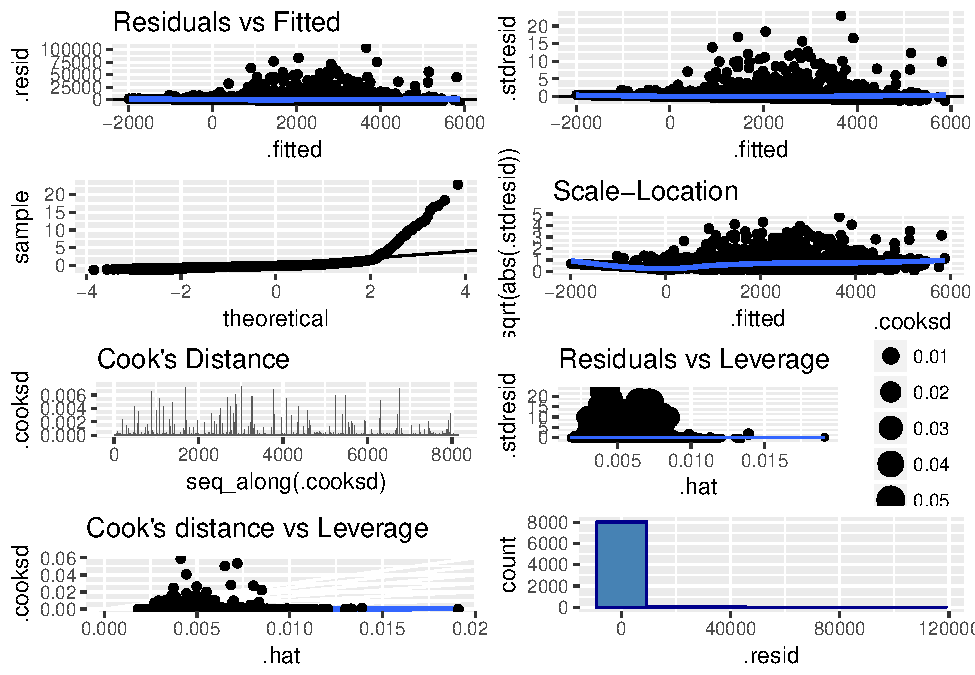
\includegraphics{DATA_621_Homework_4_files/figure-latex/lmodel-two-plots-1.pdf}

\section{4. Model Selection and
Prediction}\label{model-selection-and-prediction}

As noted in \protect\hyperlink{final-linear-model}{section 3.2.4}, I
will be using the second logistic, and second linear models for
predictions on the evaluation set.

\subsection{4.1 Transform Evaluation
Set}\label{transform-evaluation-set}

Before I proceed, I need to transform the evaluation dataset using the
same methods used for the second model.

\subsection{4.2 Split Data}\label{split-data}

\subsection{4.3 Logistic Prediction}\label{logistic-prediction}

\begin{table}[H]
\centering\rowcolors{2}{gray!6}{white}

\begin{tabular}{ll}
\hiderowcolors
\toprule
Metric & Model Results\\
\midrule
\showrowcolors
AIC & 5173.9262\\
BIC & 5419.9947\\
Deviance Diff & 1447.027\\
Accuracy & 0.7868\\
Error Rate & 0.2132\\
\addlinespace
Precision & 0.6881\\
Sensitivity & 0.3997\\
Specificity & 0.932\\
F1 Score & 0.5057\\
AUC & 0.8171\\
\bottomrule
\end{tabular}
\rowcolors{2}{white}{white}
\end{table}

\subsection{4.4 Linear Prediction}\label{linear-prediction}

\begin{longtable}[]{@{}rrrl@{}}
\toprule
actuals & predicted & error & percerror\tabularnewline
\midrule
\endhead
0 & 779.00 & -779.00 & -Inf\%\tabularnewline
2946 & 3526.21 & -580.21 & -19.69\%\tabularnewline
0 & 1684.49 & -1684.49 & -Inf\%\tabularnewline
4021 & 4869.12 & -848.12 & -21.09\%\tabularnewline
6077 & 1841.15 & 4235.85 & 69.7\%\tabularnewline
1267 & 2971.90 & -1704.90 & -134.56\%\tabularnewline
\bottomrule
\end{longtable}

As was expected the linear model performs horribly, since it didn't meet
any of the assumptions needed for regression.

\subsection{4.5 Predicting on Evaluation
Dataset}\label{predicting-on-evaluation-dataset}

\begin{verbatim}
##   Predicted_FLAG_prob Predicted_AMT Predicted_Flag
## 1           0.1355304      1198.799              0
## 2           0.2153752      1814.914              0
## 3           0.1218117      1244.482              0
## 4           0.2691361      1825.817              0
## 5           0.1536653      1286.571              0
## 6           0.2306567      2189.814              0
\end{verbatim}

\section{5. Closing Remarks}\label{closing-remarks}

Once again, the model is predicting an amount, even when the predicted
probability of an accident occuring is very low. Another problem is it's
even predicting negative amounts, which is obviously impossible!

As mentioned earlier, this dataset would require serious examination to
be used in production. I didn't want to remove the outliers, since I
believed they weren't errors in the data, but rather just extreme cases.
In retrospect, it seems I should have used some method to handle those
cases, e.g.~capping by a multiple of the IQR. Those cases were so far
from the mean and median, that they were skewing any possible
information that could have been derived from the majority of the
observations.


\end{document}
